%!TEX TS-program = xelatex
\documentclass[]{friggeri-cv}
\usepackage{afterpage}
\usepackage{hyperref}
\usepackage{color}
\usepackage{xcolor}
\usepackage{smartdiagram}
\usepackage{fontspec}
% if you want to add fontawesome package
% you need to compile the tex file with LuaLaTeX
% References:
%   http://texdoc.net/texmf-dist/doc/latex/fontawesome/fontawesome.pdf
%   https://www.ctan.org/tex-archive/fonts/fontawesome?lang=en
%\usepackage{fontawesome}
\usepackage{metalogo}
\usepackage{dtklogos}
\usepackage[utf8]{inputenc}
\usepackage{tikz}
\usetikzlibrary{mindmap,shadows}
\hypersetup{
    pdftitle={},
    pdfauthor={},
    pdfsubject={},
    pdfkeywords={},
    colorlinks=false,           % no lik border color
    allbordercolors=white       % white border color for all
}
\smartdiagramset{
    bubble center node font = \footnotesize,
    bubble node font = \footnotesize,
    % specifies the minimum size of the bubble center node
    bubble center node size = 0.5cm,
    %  specifies the minimum size of the bubbles
    bubble node size = 0.5cm,
    % specifies which is the distance among the bubble center node and the other bubbles
    distance center/other bubbles = 0.3cm,
    % sets the distance from the text to the border of the bubble center node
    distance text center bubble = 0.5cm,
    % set center bubble color
    bubble center node color = pblue,
    % define the list of colors usable in the diagram
    set color list = {lightgray, materialcyan, orange, green, materialorange, materialteal, materialamber, materialindigo, materialgreen, materiallime},
    % sets the opacity at which the bubbles are shown
    bubble fill opacity = 0.6,
    % sets the opacity at which the bubble text is shown
    bubble text opacity = 0.5,
}

\addbibresource{bibliography.bib}
\RequirePackage{xcolor}
\definecolor{pblue}{HTML}{0395DE}

\begin{document}

\header{------------  Jaziel David}{  Flores Rodríguez.}
      {Mathematical Physicist And Programmer. }
      
% Fake text to add separator      
\fcolorbox{white}{gray}{\parbox{\dimexpr\textwidth-2\fboxsep-2\fboxrule}{%
.....
}}

% In the aside, each new line forces a line break
\begin{aside}
  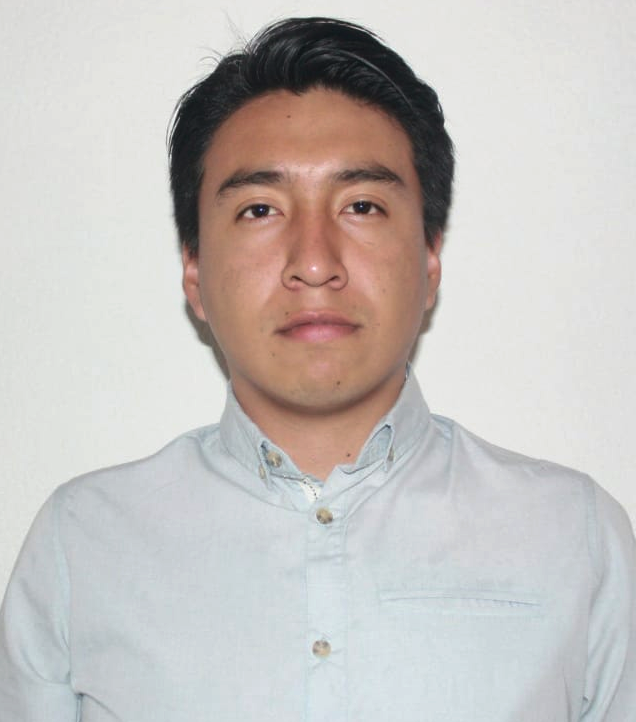
\includegraphics[width=3.9cm]{jejejejejej.png}
  \section{Tel \& LinkedIn}
    +52 55 3248 1649
    01 595 922 2525
\href{https://www.linkedin.com/in/jazzzflores/}{jazzzflores/}    
    ~
  \section{Mail}
    \href{mailto:jazzzfm@protonmail.com}{\textbf{jazzzfm@}\\protonmail.com}
    \href{mailto:jfloresr1302@alumno.ipn.mx}{\textbf{jfloresr1302@}\\alumno.ipn.mx}

    ~
  \section{Web \& Git}
    \href{https://medium.com/@jazzesfm}{JazzzFlorent.com}
   \href{https://www.hackthebox.eu/profile/171317}{hackthebox/CodexReck}
   \href{https://platzi.com/@jazzfm/}{platzi/@jazzfm}   
   \href{https://github.com/JazzzFM}{github.com/JazzzFM}
   \href{https://gitlab.com/u/JazzzFM?}{gitlab.com/JazzzFM}
    ~
 % use  \hspace{} or \vspace{} to change bubble size, if needed
  \section{Programming}
    \smartdiagram[bubble diagram]{
        \textbf{C\&C++},
        \textbf{Java},
        \textbf{Python},
        \textbf{JavaScript},
        \textbf{HTML5},
        \textbf{CSS3},
        \textbf{Bash},
        \textbf{Git}
    }
    ~
  \section{Personal Skills}
    \smartdiagram[bubble diagram]{
        \textbf{Self-}\\\textbf{Taugh},
        \textbf{Empathy},
        \textbf{Analysis},
        \textbf{renovation},
        \textbf{Proactivity},
        \textbf{Rigor},
        \textbf{Order}
    }
    ~
\end{aside}
~

\section{Education.}
\begin{entrylist}
  \entry
    {2013- 2016.}
    {Tećnico en Sistemas de Control Eléctrico.}
    {\href{https://cecyt3.ipn.mx}{<< CECyT 3 - IPN >>}}
{ \textit{Instituto Politécnico Nacional}
    }
  \entry
    {2016 - 2020}
    {Licenciatura en Física y Matemáticas.}
    {\href{https://www.esfm.ipn.mx}{<< ESFM - IPN >>}}
    {
    \textit{Instituto Politécnico Nacional}
   }
  
\end{entrylist}

\section{Experience.}
\begin{entrylist}
    
    \entry
    {2016}
    {Thesis and Final Project: }
    {\href{https://cecyt3.ipn.mx}{<< CECyT 3 - IPN >>}}
    { \textbf{Development of a Mobile-Automatic Cleaning Module.}
    \href{https://www.youtube.com/watch?v=zbDAjEfyKrY}{   \textit{<< Watch Video >>}}
    \\
    \textbf{Supervisors}: M.C. Libia Zoraida Torres e Ing. Juan Ignacio Lima Velazco.\\
    \textbf{Description}: A mobile module with a robotic arm conforms a single cleaning robot that helps the performance of household tasks, specifically sweeping and mopping, using automated mechanisms and systems \href{https://drive.google.com/file/d/12gbIxFkS-cf5gG1gvyKvA9u7UeBOZkpy/view?usp=sharing}{\textit{<< Read Thesis >>}}\\
    }
  \entry
    {2015 - 2016}
    { Social Service:}
    {\href{https://cecyt3.ipn.mx}{<< CECyT 3 - IPN >>}}
    {\textbf{Teacher Support Program of the Research Area.}
    \\
   With SolidWorks I developed gears, screws and some parts for a project that contemplated a robotic arm, I quoted the costs for the project of a drone, with the help of student researchers we designed the electronic control of engines and the interface to control a remote robot
   
   \\}
    \entry
    {2018 - 2019}
    {Part Time Teacher}
    {\href{https://www.facebook.com/Kaleido.edu/}{<< Kaleido Regualrizaciones >>}}
    {
I held the position as a teacher for students of diverse ages, teaching subjects in my area, mathematics and physics, all basic levels, but also others that were not mine, such as English, Spanish, Geography, Universal and Mexican History, Basic Financial Mathematics. I also taught in a preparation course to enter the \textbf{UNAM} University.
\href{https://drive.google.com/file/d/1w9CVCy-d3eIhm1HHeQm1GP25B_DY_1Zo/view?usp=sharing}{\textit{<< Watch Labor Certificate >>}} \\}
    \end{entrylist}

\begin{table}[h]
    \centering
        \section{Professional Goals.}
\end{table}

I am looking to work as a programmer, it could be as web developer or pentester jr. This is in a diverse, very open work area, where I can continuously grow up and learn as well as share my knowledge towards a team and offer my logical-mathematical skills always with rigor and order.

\begin{table}[h]
    \centering
    \section{Software.}
\\
    \begin{tabular}{l}

• Basic use of the GNU / Linux and Windows Operating Systems. \\
• Intermediate Terminal Use with Bash and Git. \\
• Basic use of VIM and Emacs. \\
• Basic use of HTML 5 and CSS3. \\
• Basic use of Officce and LibreOffice packages: \textbf{Excel, Word, PowerPoint}. \\
• Basic use of LaTex and Octave. \\
• Structured programming in C / C ++. \\
• Basic programming of Microcontrollers, Arduino and PLC. \\
    \end{tabular}
    \label{tab:my_label}
\end{table}
    \centering

    \newpage

\begin{aside}
~
~
~
~
~
~
    \begin{figure}
        \centering
     
\includegraphics[width=.5\textwidth,center]{CAESCOM.jpg}
\label{fig:my_label}
    \end{figure}
    ~
    ~
    \begin{figure}
        \centering
     
\includegraphics[width=.5\textwidth,center]{cin.jpeg}
     \end{figure}
    ~
    ~
    \begin{figure}
        \centering
     
\includegraphics[width=.5\textwidth,center]{CSIESCOM.png}
\label{fig:my_label}
    \end{figure}
    ~
    ~ 

     \begin{figure}
        \centering
     
\includegraphics[width=.7\textwidth,center]{ibm.png}
    \end{figure}
    ~
     \begin{figure}
        \centering
     \includegraphics[width=.44\textwidth,center]{jjajaja.png}
    \end{figure}
    ~
    \begin{figure}
        \centering
     
\includegraphics[width=.44\textwidth,center]{INSEC.png}
    \end{figure}
    ~
     \begin{figure}
        \centering
     
\includegraphics[width=.44\textwidth,center]{FUNDIBM.jpg}
    \end{figure}
      ~
     \begin{figure}
        \centering
     
\includegraphics[width=.44\textwidth,center]{BALGORI.png}
    \end{figure}
      ~
     \begin{figure}
        \centering
     
\includegraphics[width=.44\textwidth,center]{FPENTEST.png}
    \end{figure}
      ~
    \begin{figure}
        \centering
     
\includegraphics[width=.44\textwidth,center]{WATSON.png}
    \end{figure}
    
     \section{Preferred OS}
    \textbf{GNU/Linux}
\includegraphics[scale=0.40]{img/5stars.png}
    \textbf{Windows}
\includegraphics[scale=0.40]{img/3stars.png}
    \textbf{MacOS}
\includegraphics[scale=0.40]{img/2stars.png}
    ~
  \section{Languages}
    \textbf{Spanish}
\includegraphics[scale=0.40]{img/5stars.png}
    \textbf{English}
\includegraphics[scale=0.40]{img/3stars.png}
    \textbf{French}
\includegraphics[scale=0.40]{img/2stars.png}
    \textbf{Japanese}
\includegraphics[scale=0.40]{img/1stars.png}
    

\end{aside}

\section{Extra-Academic Courses}
\begin{entrylist}
 
  \entry{ 2019 - 1 }{Club de Algoritmia de ESCOM}{\href{https://www.cec.escom.ipn.mx/index.php/es/}{<< ESCOM - IPN >>}}{
I was a member from February to May of this year, where we study deeper topics such as \textit{Dynamic programming} and \textit{Backtracking}}
  
  \entry{ 07/2019 }{Summer School of Mathematics}
  {\href{https://www.math.cinvestav.mx}{<< CINVESTAV - IPN >>}}
  {
  The last summer vacations I decided to go because I was interested in recent topics in mathematics and it was a great opportunity to know the work of others and that great institution. I was particularly interested in areas like \textit{Cryptography} and the \textit{Super Computation}, but also the \textit{Topology} and \textit {Algebra}.
   << \href{https://drive.google.com/file/d/0BxsBj4oBVw3fMlVjQXlfOGl3VHhYUm15RlRlQXVHMHE1Nm9Z/view?usp=sharing}{\textit{See Certificate}} >>
  }
  
  \entry{2019 - 2}{Club de Seguridad Informática de ESCOM}{\href{https://www.cec.escom.ipn.mx/index.php/es/}{<< ESCOM - IPN >>}}
  {
 Active member of three kinds of activities; \textit{Introduction to Computer Security}, \textit{Pentesting} and \textit{Capture the Flag}, it was here that I have opened up opportunities for collaboration with other students in an amazing meetup in platzi as well as starting the Hacker culture and create an account on HackTheBox to perform penetration tests and challenges}
  
  \entry{13/09/2019}{Watson Studio Workshop - IBM Day}{\href{https://www.cec.escom.ipn.mx/index.php/es/}{<< ESCOM - IPN>>}}
  {I take an introductory workshop on Watson Artificial Intelligence where we made algorithm configurations for; categorize a data set, image recognition and creation of a very basic chatbot, as well as understand the principles of its operation.\href{https://drive.google.com/file/d/1HZNd6Rm6PFyitDFkMpKJaU-E61z-BiQa/view?usp=sharing}{ << See Here >>}
  }
  
   \entry{23/09/2019}{Introduction to Terminal and Command Line }{\href{https://platzi.com}{<< Platzi >>}}
  {
  I learned to use the UNIX terminal.
  \href{https://drive.google.com/file/d/1mlRopoqhOzYW9gVK44IMv5gWyx7ri1Oq/view?usp=sharing}{ << See Certificate >>}
  }
  \entry{16/10/2019}{ Introduction to Cyber Security
 }{\href{https://platzi.com}{<< Platzi >>}}
  {In this course I understood the basic fundamentals of Cyber Security, such as protocols, regulations like TCP/IP or OSI, firewalls, honeypots, etc.
  \href{https://drive.google.com/file/d/1rxih1q_8NExuBfgGRTgl7nB13LWx3TEf/view?usp=sharing}{<< See Certificate >>}
  }
 
  \entry{16/10/2019}{
IBM Cloud Basics
 }{\href{https://platzi.com}{<< Platzi >>}}
  {I understood how to start in cloud computing on the side of IBM and its catalog of services such as deploy applications, economy of APIs or cognitive solutions using Watson. \href{https://drive.google.com/file/d/1rtJuI9LZY-5HCclYUGmYYYGadnAICH3D/view?usp=sharing}{<<  See Certificate >>}
  }

\entry{24/12/2019}{
Basic Algorithm Course
 }{\href{https://platzi.com}{<< Platzi >>}}
 {I learned to implement data structures such as queues, stacks, trees and graphs, as well as basic search and ordering algorithms.
  \href{https://drive.google.com/file/d/1YMPauE56JO_EAAnPZ4PvS5xyCPK-3MMs/view?usp=sharing}{<<  See Certificate >>}
  }
  
  \entry{31/12/2019}{
Pentesting Fundamentals Course
 }{\href{https://platzi.com}{<< Platzi >>}}
  {I understood the protocols behind an nmap scan, learned the basics of metasploit, and the phases of pentesting as well as what a report should carry. \href{https://drive.google.com/file/d/1FMRABdPX0U9CDHdARuaY6e60bueEHbId/view?usp=sharing}{<<  See Certificate >>}
  }
\end{entrylist}



\section{Personal Comments}
\justify
I like to write and read, in general, create. I am interested in mathematics as a creative activity, as if it were literature, I think about doing a postgraduate degree in \textit{Number Theory}, \textit{Cryptography}, \textit{Super Computation} or \textit{Topology} in CINVESTAV or in other countries, however, at this moment I am interested in knowing the industry and developing in it before at least three continuous years.

\end{document}
